% Author: Izaak Neutelings (July 2018)
\documentclass[border=3pt,tikz]{standalone}
\usepackage{tikz}
\tikzset{>=latex} % for LaTeX arrow head
\usepackage{xcolor}
\colorlet{charge+}{red!90!white}
\colorlet{charge-}{blue!80!white}
%\colorlet{metal}{black!5}
%\colorlet{silk}{blue!40!red!10}
%\colorlet{plastic}{yellow!70!red!20}
%\colorlet{glas}{blue!4}
%\usetikzlibrary{positioning,calc}
\tikzstyle{rod}=[top color=white,bottom color=black!20,shading angle=5]
\tikzstyle{glas}=[top color=blue!4,bottom color=blue!15,shading angle=120]
\tikzstyle{silk}=[top color=blue!40!red!10,bottom color=blue!40!red!30,shading angle=30]
\tikzstyle{metal}=[top color=black!5,bottom color=black!15,shading angle=30]
\def\L{4.5}
\def\W{0.5}
\def\N{8}
\def\angle{45}

\def\chargedRod{
  \draw[glas,shading angle=45,rotate=\angle] (0,0) rectangle ++(\L,\W);
  \foreach \i [evaluate={\x=\i*\L/(\N+1);}] in {1,...,\N}{
    \path[rotate=\angle] (0,\W/2) --++(\x,0) node[charge+] {+};
  }
}

\def\ground{
  \foreach \i [evaluate={\y=-0.12*(\i-1); \w=1.1-0.25*\i); \x=-\w/2;}] in {1,...,4}{
    \draw[thick] (G) ++ (\x,\y) --++ (\w,0);
  }
}

\begin{document}
\Large



% CHARGED INSULATORS BY RUBBING B
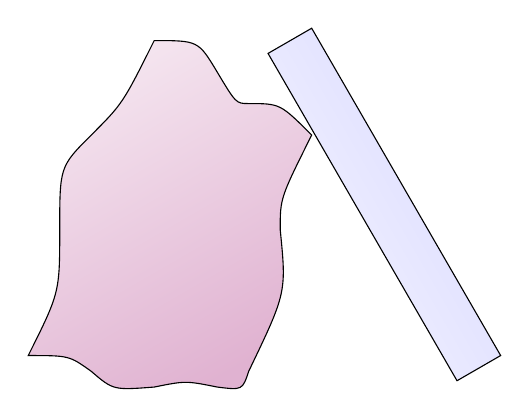
\begin{tikzpicture}[scale=0.4]
  \def\angle{120}
  \def\L{12}
  \def\W{1.6}
  \def\N{7}
  
  %\draw[very thin,color=gray] (-2,-2) grid (10,10);
  \coordinate (SW)  at (   0,  0   ); % SOUTH WEST
  \coordinate (WC1) at (   1,  2   );
  \coordinate (W1)  at (   1,  4   );
  \coordinate (WC2) at (   1,  6   );
  \coordinate (W2)  at (   2,  7   );
  \coordinate (WC3) at (   3,  8   );
  \coordinate (NW)  at (   4, 10   ); % NORTH WEST
  \coordinate (NC1) at ( 5.4, 10   );
  \coordinate (N1)  at (   6,  9   );
  \coordinate (NC2) at ( 6.6,  8   );
  \coordinate (N2)  at (   7,  8   );
  \coordinate (NC3) at (   8,  8   );
  \coordinate (NE)  at (   9,  7   ); % NORTH EAST
  \coordinate (EC1) at (   8,  5   );
  \coordinate (E1)  at (   8,  4   );
  \coordinate (EC2) at ( 8.2,  2   );
  \coordinate (E2)  at (   7, -0.5 );
  \coordinate (EC3) at ( 6.8, -1.1 );
  \coordinate (SE)  at (   6, -1   ); % SOUTH EAST
  \coordinate (SC1) at (   5, -0.8 );
  \coordinate (S1)  at (   4, -1   );
  \coordinate (SC2) at ( 2.7, -1.1 );
  \coordinate (S2)  at (   2, -0.5 );
  \coordinate (SC3) at ( 1.3,  0   );
  
  % SILK
  \draw[silk]
    (SW) .. controls (WC1) .. (W1) % SOUTH WEST
         .. controls (WC2) .. (W2)
         .. controls (WC3) .. (NW) % NORTH WEST
         .. controls (NC1) .. (N1)
         .. controls (NC2) .. (N2)
         .. controls (NC3) .. (NE) % NORTH EAST
         .. controls (EC1) .. (E1)
         .. controls (EC2) .. (E2)
         .. controls (EC3) .. (SE) % SOUTH EAST
         .. controls (SC1) .. (S1)
         .. controls (SC2) .. (S2)
         .. controls (SC3) .. cycle;
  
  % ROD
  \coordinate (O) at (15,0);
  \draw[glas,rotate around={\angle:(O)}] (O) rectangle ++(\L,\W);
  
%  \draw[dashed,very thin]
%    (SW) -- (WC1) -- (W1) -- (WC2) -- (W2) -- (WC3) --
%    (NW) -- (NC1) -- (N1) -- (NC2) -- (N2) -- (NC3) --
%    (NE) -- (EC1) -- (E1) -- (EC2) -- (E2) -- (EC3) --
%    (SE) -- (SC1) -- (S1) -- (SC2) -- (S2) -- (SC3) -- cycle;
%  
%  \foreach \p in {(SW), (WC1), (W1), (WC2), (W2), (WC3),
%                  (NW), (NC1), (N1), (NC2), (N2), (NC3),
%                  (NE), (EC1), (E1), (EC2), (E2), (EC3),
%                  (SE), (SC1), (S1), (SC2), (S2), (SC3)}{
%    \fill \p circle (2pt) node[above,scale=0.3] {\p};
%  }
\end{tikzpicture}

% CHARGED INSULATORS BY RUBBING B
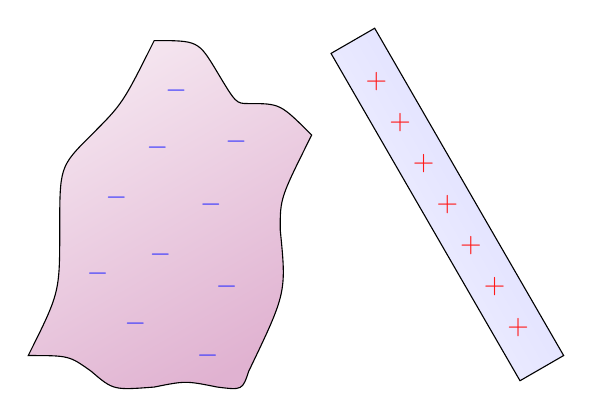
\begin{tikzpicture}[scale=0.4]
  \def\angle{120}
  \def\L{12}
  \def\W{1.6}
  \def\N{7}
  
  \coordinate (SW)  at (   0,  0   ); % SOUTH WEST
  \coordinate (WC1) at (   1,  2   );
  \coordinate (W1)  at (   1,  4   );
  \coordinate (WC2) at (   1,  6   );
  \coordinate (W2)  at (   2,  7   );
  \coordinate (WC3) at (   3,  8   );
  \coordinate (NW)  at (   4, 10   ); % NORTH WEST
  \coordinate (NC1) at ( 5.4, 10   );
  \coordinate (N1)  at (   6,  9   );
  \coordinate (NC2) at ( 6.6,  8   );
  \coordinate (N2)  at (   7,  8   );
  \coordinate (NC3) at (   8,  8   );
  \coordinate (NE)  at (   9,  7   ); % NORTH EAST
  \coordinate (EC1) at (   8,  5   );
  \coordinate (E1)  at (   8,  4   );
  \coordinate (EC2) at ( 8.2,  2   );
  \coordinate (E2)  at (   7, -0.5 );
  \coordinate (EC3) at ( 6.8, -1.1 );
  \coordinate (SE)  at (   6, -1   ); % SOUTH EAST
  \coordinate (SC1) at (   5, -0.8 );
  \coordinate (S1)  at (   4, -1   );
  \coordinate (SC2) at ( 2.7, -1.1 );
  \coordinate (S2)  at (   2, -0.5 );
  \coordinate (SC3) at ( 1.3,  0   );
  
  % SILK
  \draw[silk]
    (SW) .. controls (WC1) .. (W1) % SOUTH WEST
         .. controls (WC2) .. (W2)
         .. controls (WC3) .. (NW) % NORTH WEST
         .. controls (NC1) .. (N1)
         .. controls (NC2) .. (N2)
         .. controls (NC3) .. (NE) % NORTH EAST
         .. controls (EC1) .. (E1)
         .. controls (EC2) .. (E2)
         .. controls (EC3) .. (SE) % SOUTH EAST
         .. controls (SC1) .. (S1)
         .. controls (SC2) .. (S2)
         .. controls (SC3) .. cycle;
  \foreach \p in {(4.7,8.4), (6.6,6.8),
                  (4.1,6.6), (5.8,4.8),
                  (2.8,5.0), (4.2,3.2), (6.3,2.2),
                  (2.2,2.6), (3.4,1.0), (5.7,0.0)}{
    \node[charge-] at \p {$-$};
  }
  
  % ROD
  \coordinate (O) at (17,0);
  \draw[glas,rotate around={\angle:(O)}] (O) rectangle ++(\L,\W);
  \foreach \i [evaluate={\x=\i*\L/(\N+1);}] in {1,...,\N}{
    \path[rotate around={\angle:(O)}] (O) ++ (0,\W/2) --++(\x,0) node[charge+] {+};
  }
  
\end{tikzpicture}



% CHARGE BY CONDUCTION A

\begin{tikzpicture}
  \draw[rod] (0,0) rectangle ++(\L,\W) node[charge+,midway] {$+\,+\,+\,+\,+\,+\,+\,\,+$};
  \draw[rod] (\L+4,0) rectangle ++(\L,\W);
\end{tikzpicture}

% CHARGE BY CONDUCTION B

\begin{tikzpicture}
  \draw[rod] (0,0) rectangle ++(\L,\W) node[charge+,midway] {$+\quad\, +\quad\, +\quad\,\, +$};
  \draw[rod] (\L,0) rectangle ++(\L,\W) node[charge+,midway] {$+\quad\, +\quad\, +\quad\,\, +$};
\end{tikzpicture}

% CHARGE BY CONDUCTION C

\begin{tikzpicture}
  \draw[rod] (0,0) rectangle ++(\L,\W) node[charge+,midway] {$+\quad\, +\quad\, +\quad\,\, +$};
  \draw[rod] (\L+4,0) rectangle ++(\L,\W) node[charge+,midway] {$+\quad\, +\quad\, +\quad\,\, +$};
\end{tikzpicture}



% CHARGE BY INDUCTION A
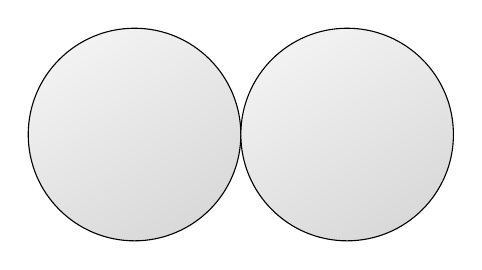
\begin{tikzpicture}
  \def\R{0.3*\L}
  \coordinate (A) at (0,0);
  \coordinate (B) at (2*\R,0);
  \draw[metal] (A) circle (\R);
  \draw[metal] (B) circle (\R);
\end{tikzpicture}

% CHARGE BY INDUCTION B
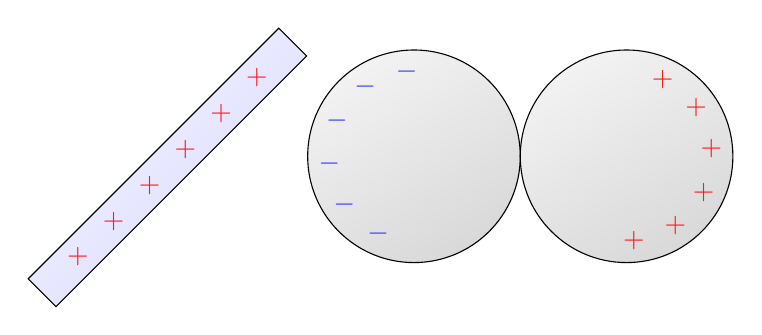
\begin{tikzpicture}
  \def\R{0.3*\L}
  \def\N{6}
  \coordinate (A) at ({1.01*\R+\L*cos(\angle)},{0.6*\L*sin(\angle)});
  \coordinate (B) at ({3.01*\R+\L*cos(\angle)},{0.6*\L*sin(\angle)});
  \chargedRod
  \draw[metal] (A) circle (\R);
  \draw[metal] (B) circle (\R);
  \foreach \i [evaluate={\a=170-30*(\N-1)/2+30*(\i-1);}] in {1,...,\N}{
    \path (A) --++ (\a:0.8*\R) node[charge-] {$-$};
    \path (B) --++ (\a-180:0.8*\R) node[charge+] {$+$};
  }
\end{tikzpicture}

% CHARGE BY INDUCTION C
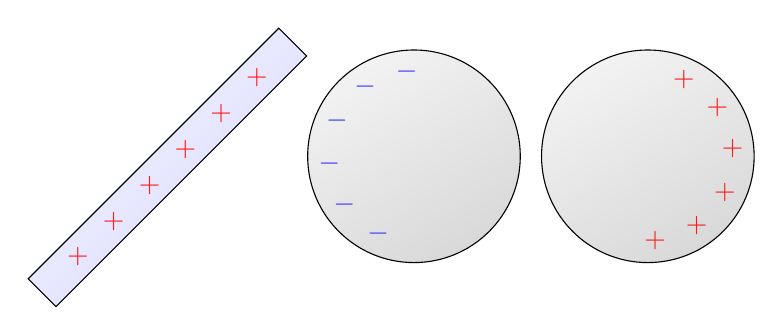
\begin{tikzpicture}
  \def\R{0.3*\L}
  \def\N{6}
  \coordinate (A) at ({1.01*\R+\L*cos(\angle)},{0.6*\L*sin(\angle)});
  \coordinate (B) at ({3.21*\R+\L*cos(\angle)},{0.6*\L*sin(\angle)});
  \chargedRod
  \draw[metal] (A) circle (\R);
  \draw[metal] (B) circle (\R);
  \foreach \i [evaluate={\a=170-30*(\N-1)/2+30*(\i-1);}] in {1,...,\N}{
    \path (A) --++ (\a:0.8*\R) node[charge-] {$-$};
    \path (B) --++ (\a-180:0.8*\R) node[charge+] {$+$};
  }
\end{tikzpicture}

% CHARGE BY INDUCTION B
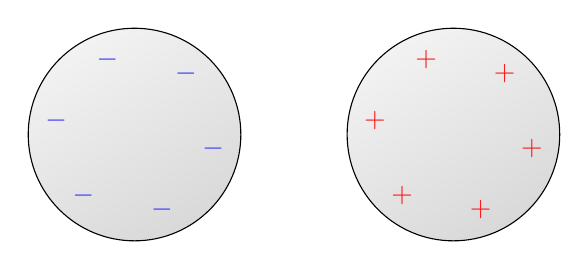
\begin{tikzpicture}
  \def\R{0.3*\L}
  \def\N{6}
  \coordinate (A) at (0,0);
  \coordinate (B) at (3.0*\R,0);
  \draw[metal] (A) circle (\R);
  \draw[metal] (B) circle (\R);
  \foreach \i [evaluate={\a=-10+360*\i/\N;}] in {1,...,\N}{
    \path (A) --++ (\a:0.75*\R) node[charge-] {$-$};
    \path (B) --++ (\a:0.75*\R) node[charge+] {$+$};
  }
\end{tikzpicture}



% CHARGE BY INDUCTION & GROUNDING A
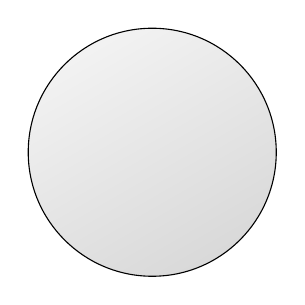
\begin{tikzpicture}
  \def\R{0.35*\L}
  \draw[metal] (0,0) circle (\R);
\end{tikzpicture}

% CHARGE BY INDUCTION & GROUNDING B
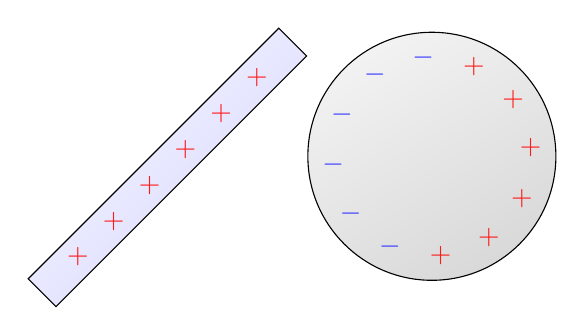
\begin{tikzpicture}
  \def\R{0.35*\L}
  \def\N{6}
  \def\h{0.6*\L*sin(\angle)}
  \coordinate (O) at ({1.01*\R+\L*cos(\angle)},{\h});
  \chargedRod
  \draw[metal] (O) circle (\R);
  \foreach \i [evaluate={\a=170-30*(\N-1)/2+30*(\i-1);}] in {1,...,\N}{
    \path (O) --++ (\a:0.8*\R) node[charge-] {$-$};
    \path (O) --++ (\a-180:0.8*\R) node[charge+] {$+$};
  }
\end{tikzpicture}

% CHARGE BY INDUCTION & GROUNDING C
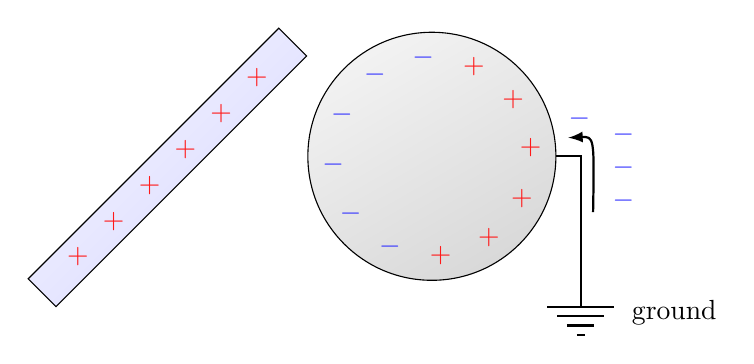
\begin{tikzpicture}
  \def\R{0.35*\L}
  \def\N{6}
  \def\h{0.6*\L*sin(\angle)}
  \coordinate (O) at ({1.01*\R+\L*cos(\angle)},{\h});
  
  % ROD & SPHERE
  \chargedRod
  \draw[metal] (O) circle (\R);
  \foreach \i [evaluate={\a=170-30*(\N-1)/2+30*(\i-1);}] in {1,...,\N}{
    \path (O) --++ (\a:0.8*\R) node[charge-] {$-$};
    \path (O) --++ (\a-180:0.8*\R) node[charge+] {$+$};
  }
  
  % GROUND
  \draw[thick] (O) ++ (\R,0) --++ (0.2*\R,0) coordinate (P) --++ (0,{-\h}) coordinate (G);
  \node[below=2,right=15] at (G) {ground};
  \ground
  
  % ELECTRONS
  \draw[->,thick] (P) ++ (0.1*\R,-0.45*\R)
                  .. controls ++(0.01*\R,0.61*\R) .. ++(-0.2*\R,0.6*\R) node[charge-,right=4,above] {$-$};
  \node[charge-,below=4,right=8,align=center] at (P) {$-$\\$-$\\$-$};
  
\end{tikzpicture}

% CHARGE BY INDUCTION & GROUNDING D
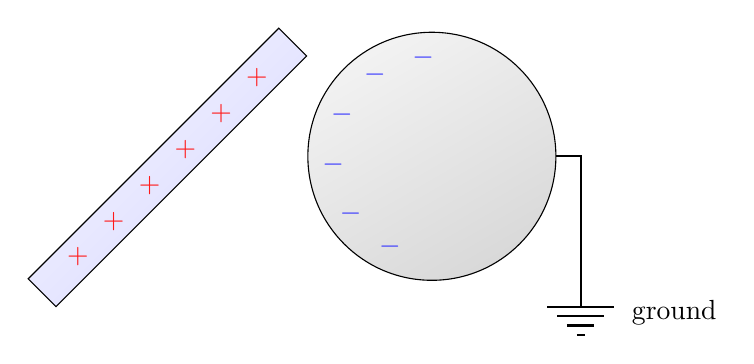
\begin{tikzpicture}
  \def\R{0.35*\L}
  \def\N{6}
  \def\h{0.6*\L*sin(\angle)}
  \coordinate (O) at ({1.01*\R+\L*cos(\angle)},{\h});
  
  % ROD & SPHERE
  \chargedRod
  \draw[metal] (O) circle (\R);
  \foreach \i [evaluate={\a=170-30*(\N-1)/2+30*(\i-1);}] in {1,...,\N}{
    \path (O) --++ (\a:0.8*\R) node[charge-] {$-$};
  }
  
  % GROUND
  \draw[thick] (O) ++ (\R,0) --++ (0.2*\R,0) --++ (0,{-\h}) coordinate (G);
  \node[below=2,right=15] at (G) {ground};
  \ground
\end{tikzpicture}

% CHARGE BY INDUCTION & GROUNDING E
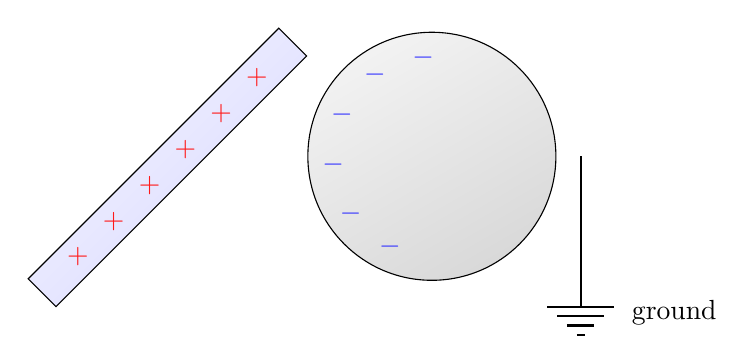
\begin{tikzpicture}
  \def\R{0.35*\L}
  \def\N{6}
  \def\h{0.6*\L*sin(\angle)}
  \coordinate (O) at ({1.01*\R+\L*cos(\angle)},{\h});
  
  % ROD & SPHERE
  \chargedRod
  \draw[metal] (O) circle (\R);
  \foreach \i [evaluate={\a=170-30*(\N-1)/2+30*(\i-1);}] in {1,...,\N}{
    \path (O) --++ (\a:0.8*\R) node[charge-] {$-$};
  }
  
  % GROUND
  \draw[thick] (O) ++ (1.2*\R,0) --++ (0,{-\h}) coordinate (G);
  \node[below=2,right=15] at (G) {ground};
  \ground
\end{tikzpicture}

% CHARGE BY INDUCTION & GROUNDING F
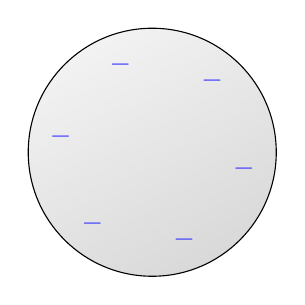
\begin{tikzpicture}
  \def\R{0.35*\L}
  \def\N{6}
  \def\h{0.6*\L*sin(\angle)}
  \coordinate (O) at ({1.01*\R+\L*cos(\angle)},{\h});
  
  % ROD & SPHERE
  \draw[metal] (O) circle (\R);
  \foreach \i [evaluate={\a=-10+360*\i/\N;}] in {1,...,\N}{
    \path (O) --++ (\a:0.75*\R) node[charge-] {$-$};
  }
  
\end{tikzpicture}



\end{document}